\documentclass[10pt]{beamer}

\usetheme[progressbar=frametitle]{metropolis}
\usepackage{appendixnumberbeamer}

\usepackage{amsfonts}
\usepackage{amssymb}
\usepackage{amsthm}
\usepackage{amsmath}
\usepackage{amsopn} 

\usepackage{wrapfig}

\usepackage{booktabs}
\usepackage[scale=2]{ccicons}

\usepackage{pgfplots}
\usepgfplotslibrary{dateplot}

\usepackage{xspace}
\newcommand{\themename}{\textbf{\textsc{metropolis}}\xspace}

\title{Understanding the reflectance of homo-polymers using White Light Spectroscopic Reflectometry}
\subtitle{Ongoing Master Thesis}
% \date{\today}
\date{}
\author{Nathan Hugh Barr}
\institute{Roskilde University}
% \titlegraphic{\hfill\includegraphics[height=1.5cm]{logo.pdf}}

\begin{document}

\maketitle

\begin{frame}{Table of contents}
  \setbeamertemplate{section in toc}[sections numbered]
  \tableofcontents[hideallsubsections]
\end{frame}

	\section{Master Thesis Background}

	\begin{frame}{Master Thesis Background}

CHESS Dec 17 and May 18

[Insert Photos]

	\end{frame}

	\begin{frame}{Thin Film Thickness}
	
	\begin{minipage}{0.47\textwidth}
	    \begin{itemize}
	    \item Experimental techniques: Atomic Force Microscopy, Ellipsometry and x-ray reflectometry
	    \item Spectroscopic Reflectometry
	    \begin{itemize}
	    \item In-situ
	    \item Harsh environment
	    \item Small enough for test chamber and testing stage
	    \end{itemize}
	    \item Complement GISAXS measurements 
	    \end{itemize}
	\end{minipage}
	\begin{minipage}{0.5\textwidth}
	    \begin{figure}
	    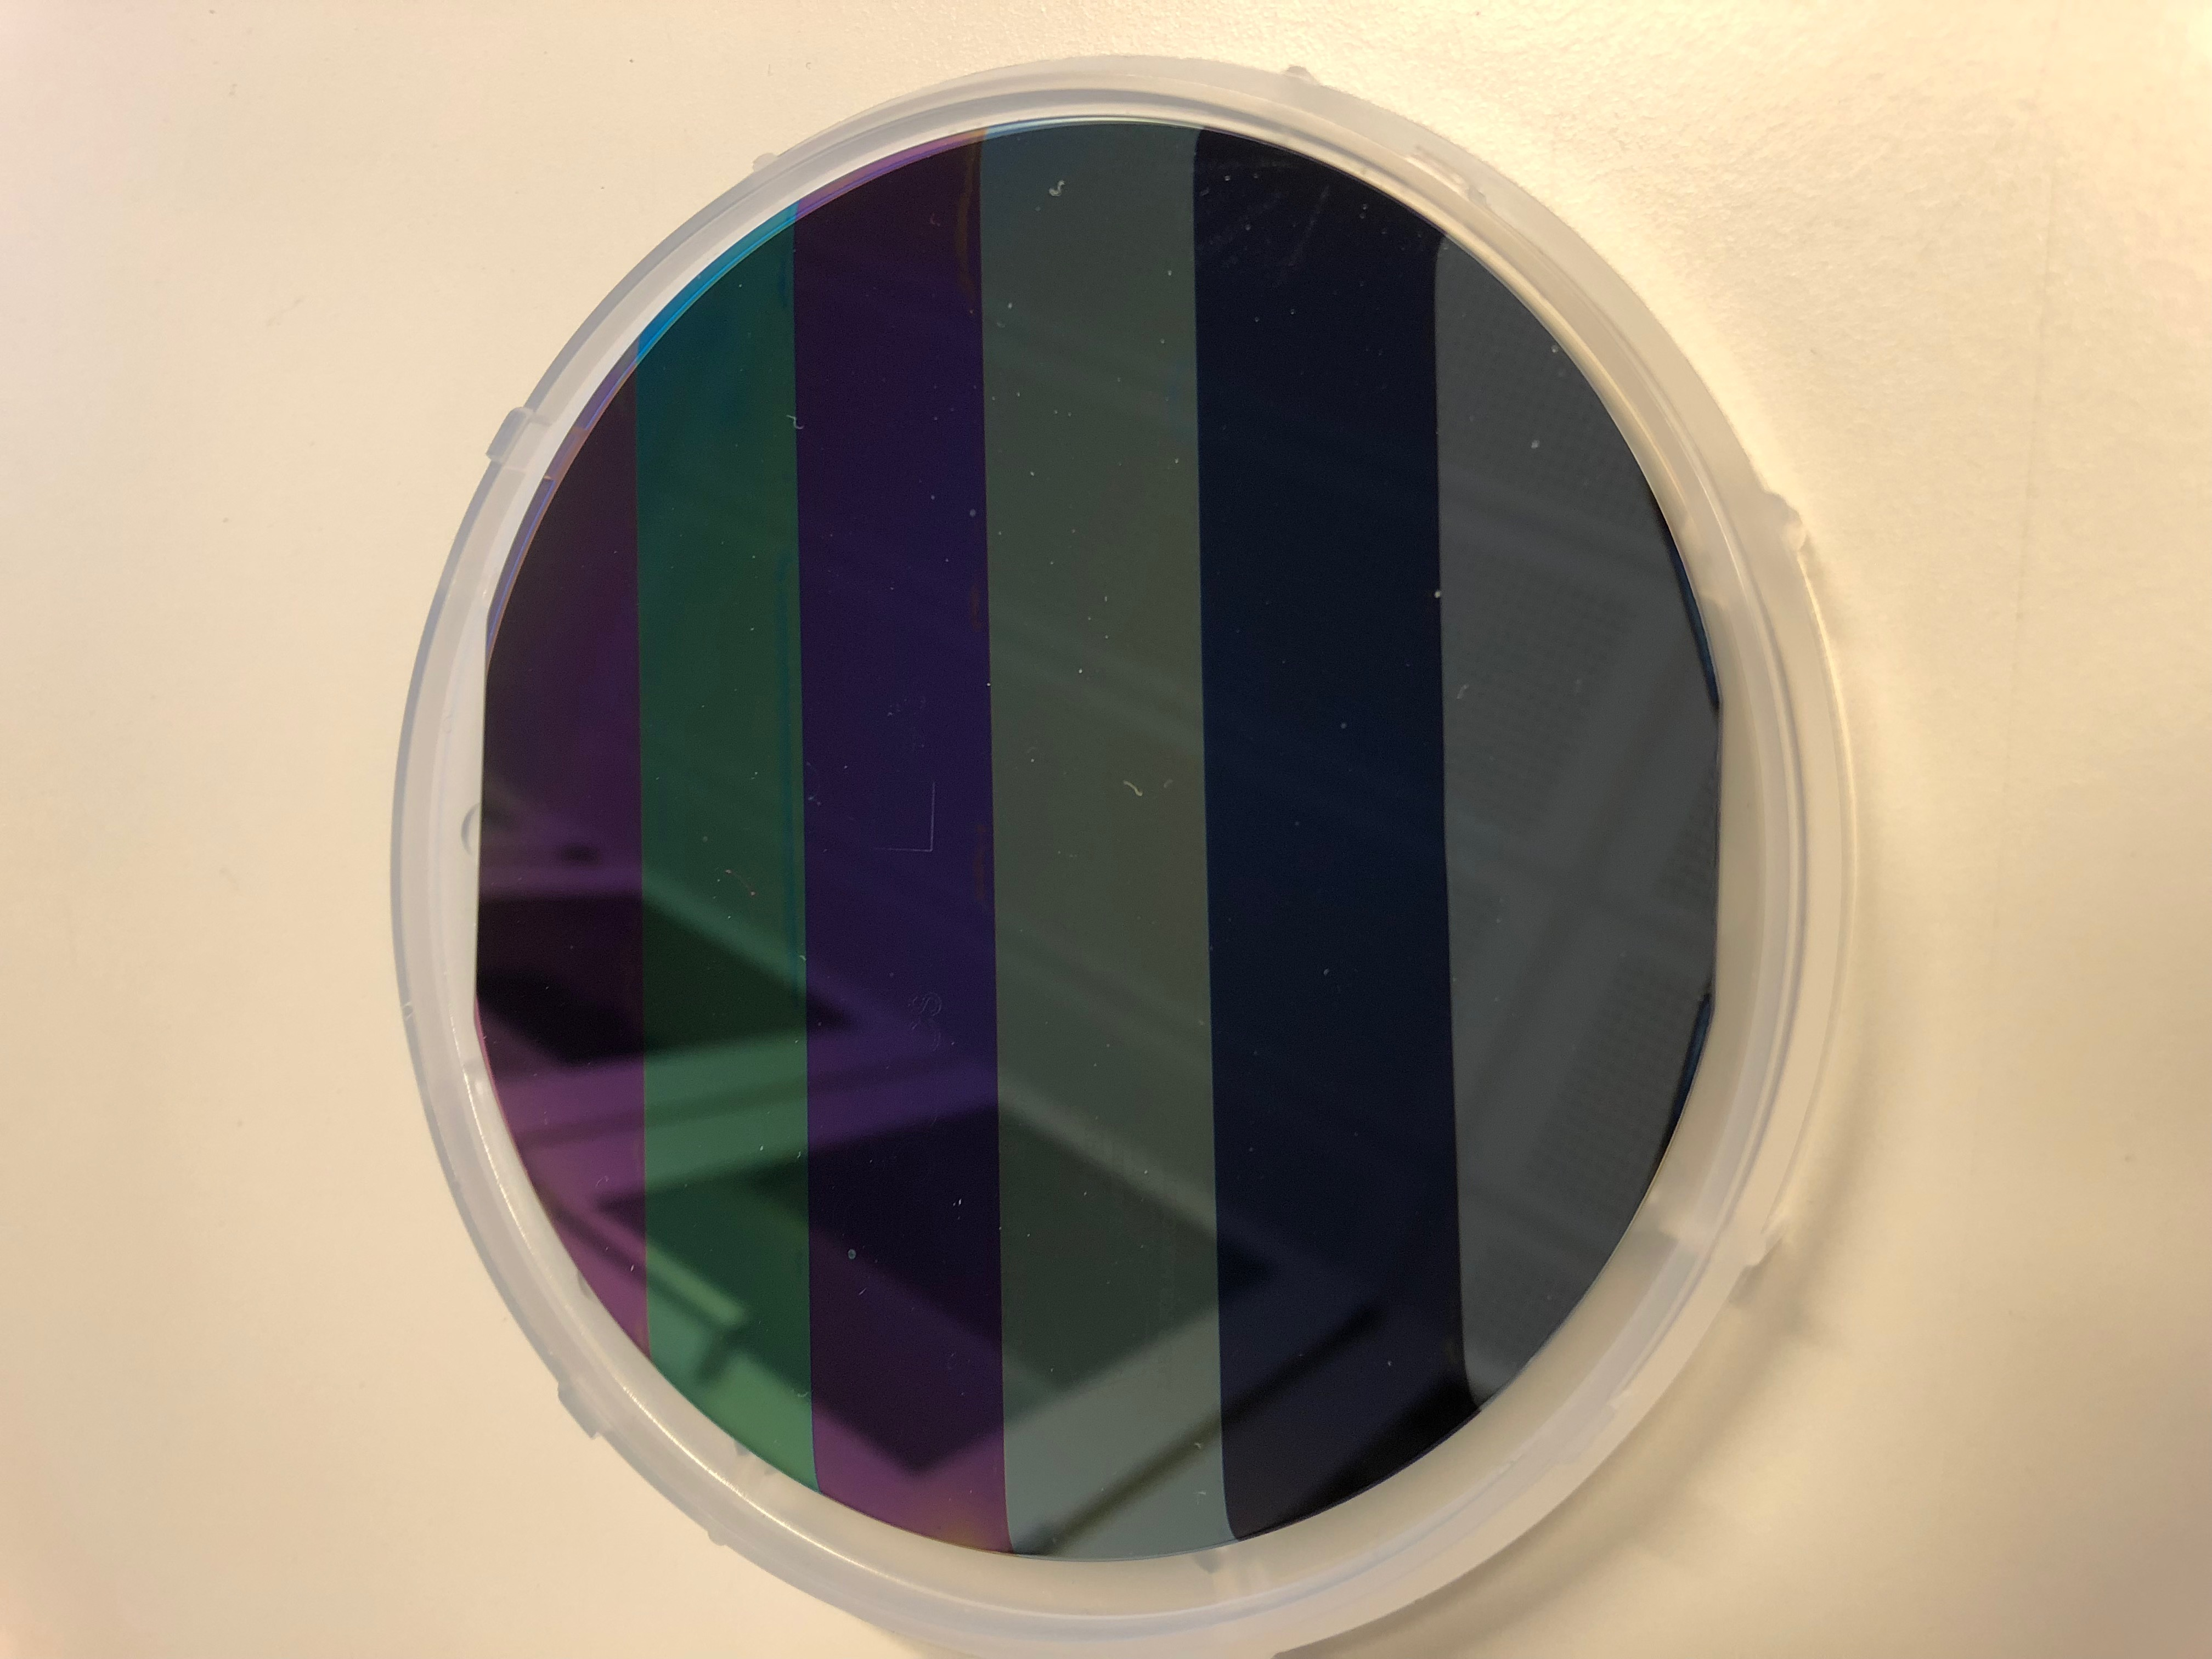
\includegraphics[scale=0.025,angle=-90]{stepwafer.JPG}
	    \end{figure}
	\end{minipage}
	
 
	\end{frame}
	
	\section{Experimental Setup}
	
	\begin{frame}{Components}
	NanoCalc XR,Halogen Light Source, Test Chamber and Single Point Stage
	
	\begin{minipage}{0.47\textwidth}
	\begin{figure}
	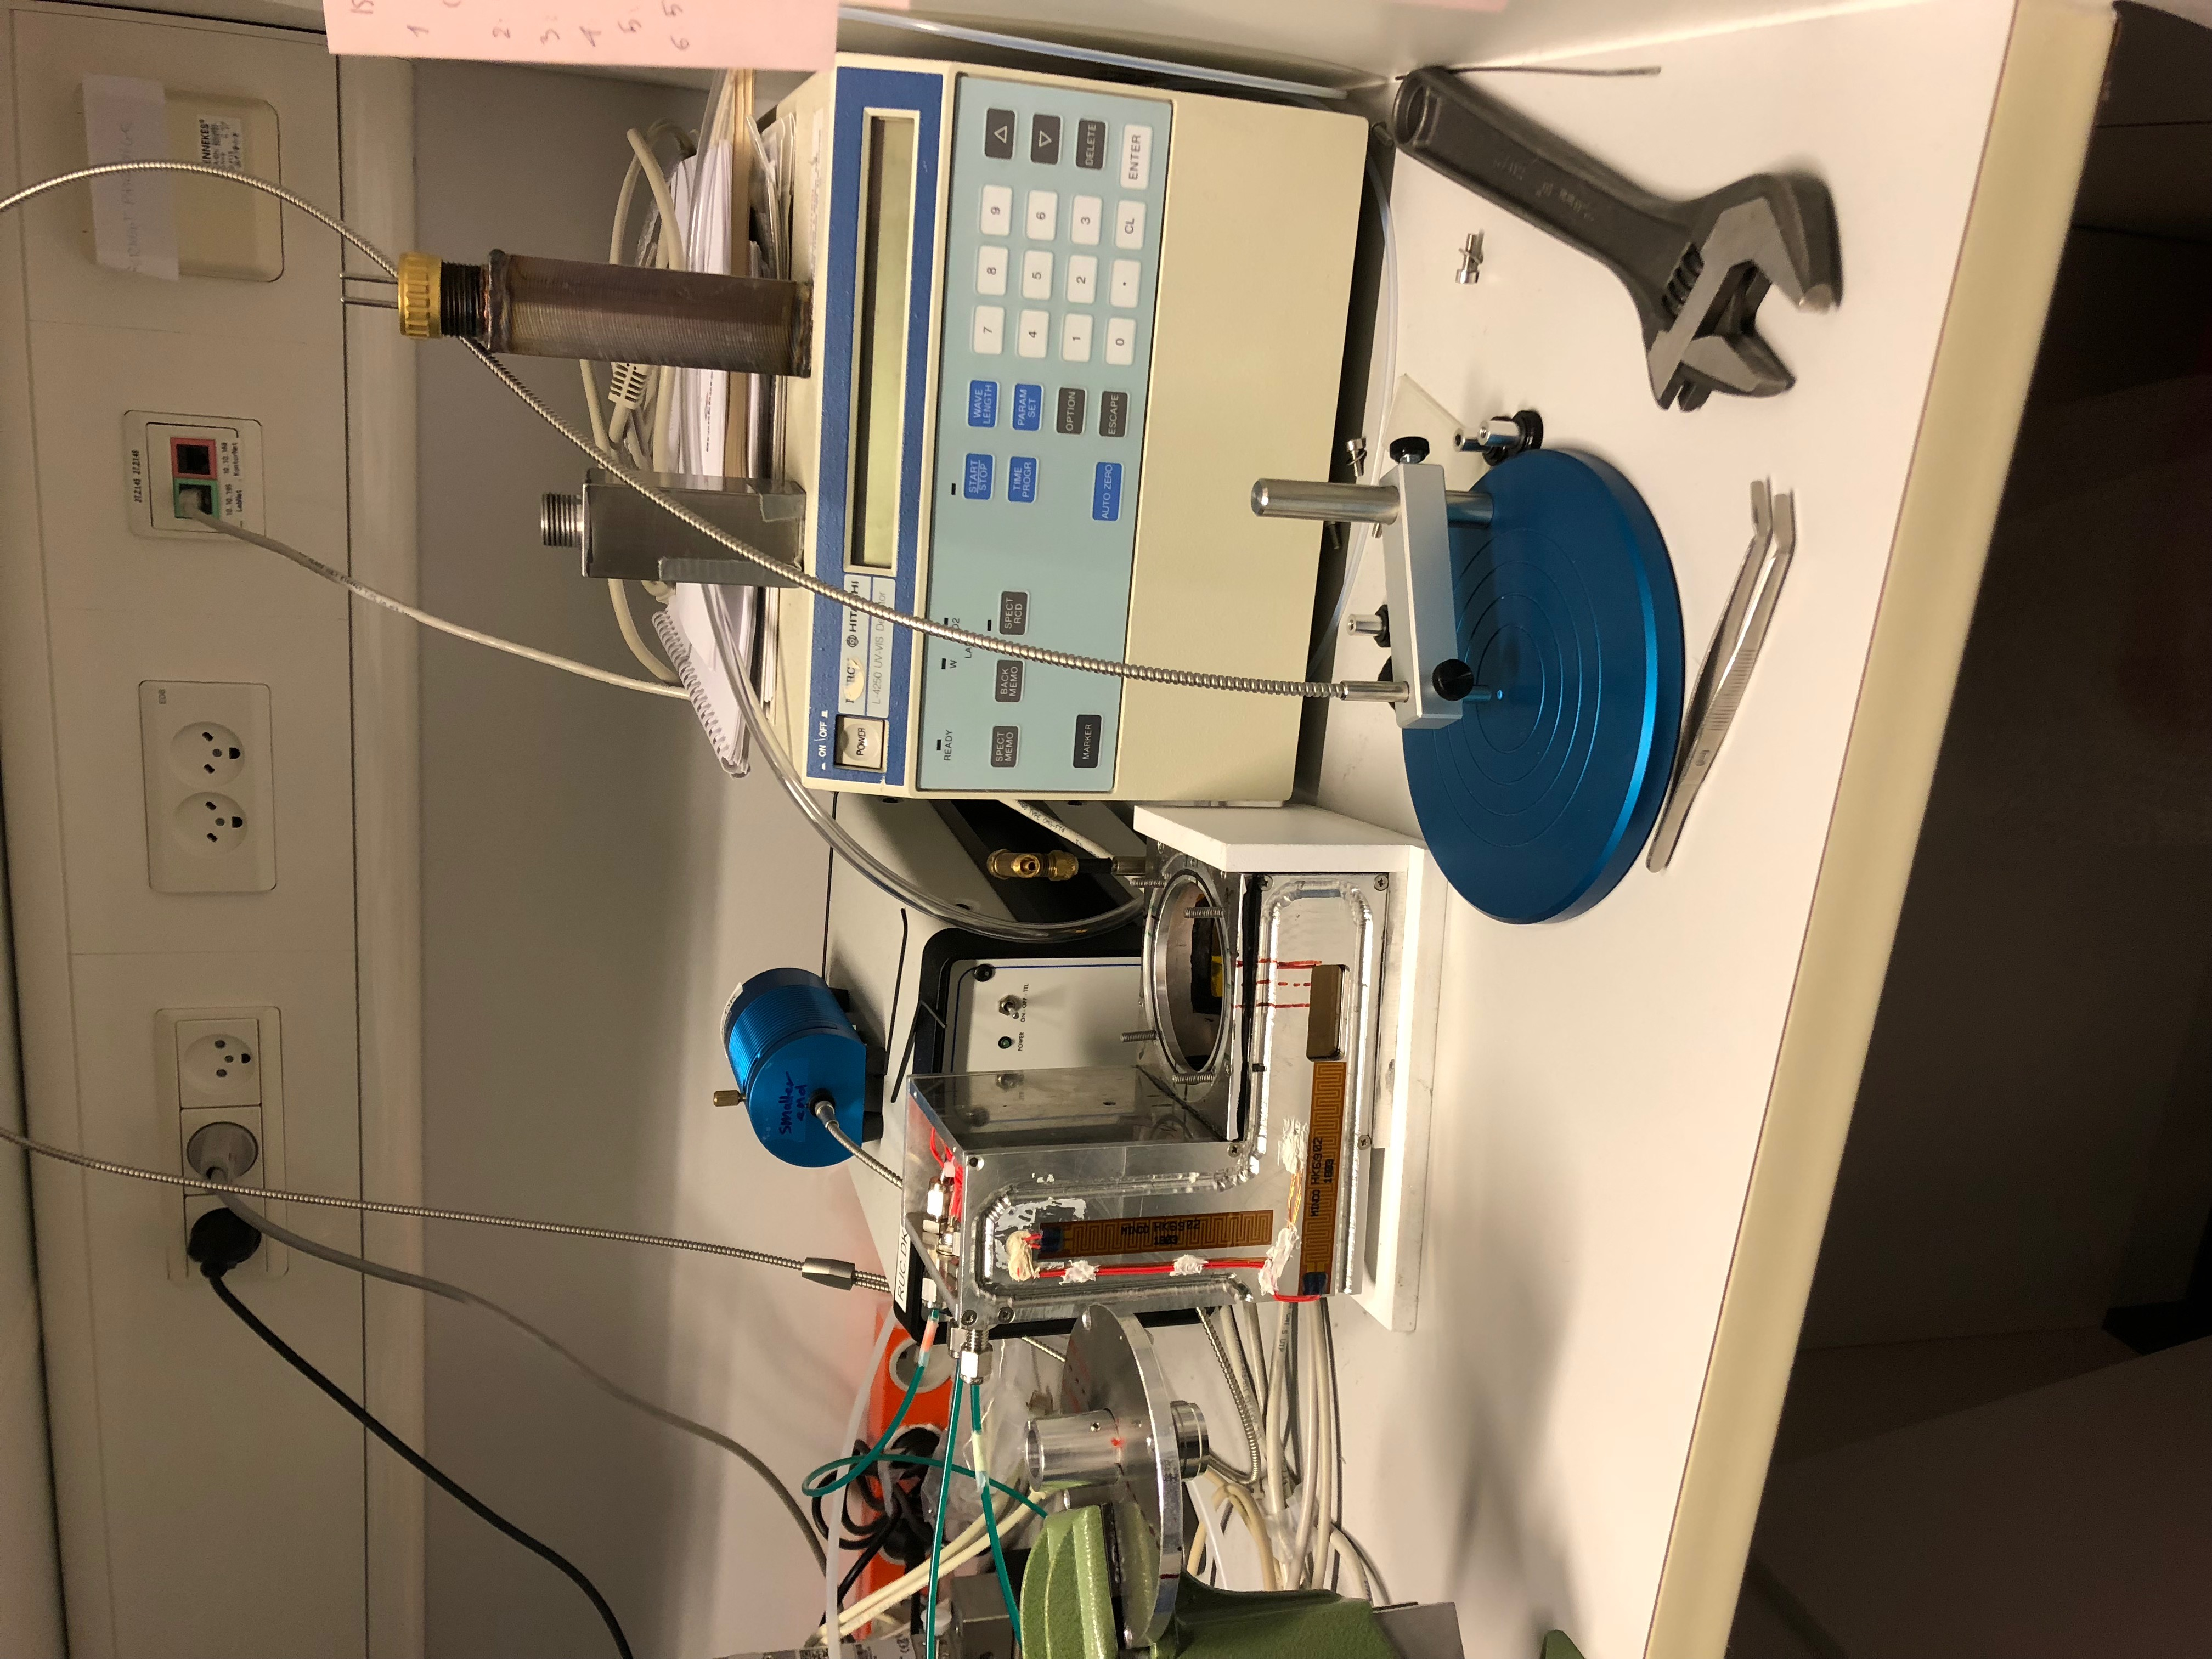
\includegraphics[scale=0.04,angle=-90]{setup1.JPG}
	\end{figure}
	\end{minipage}
	\begin{minipage}{0.5\textwidth}
	\begin{figure}
	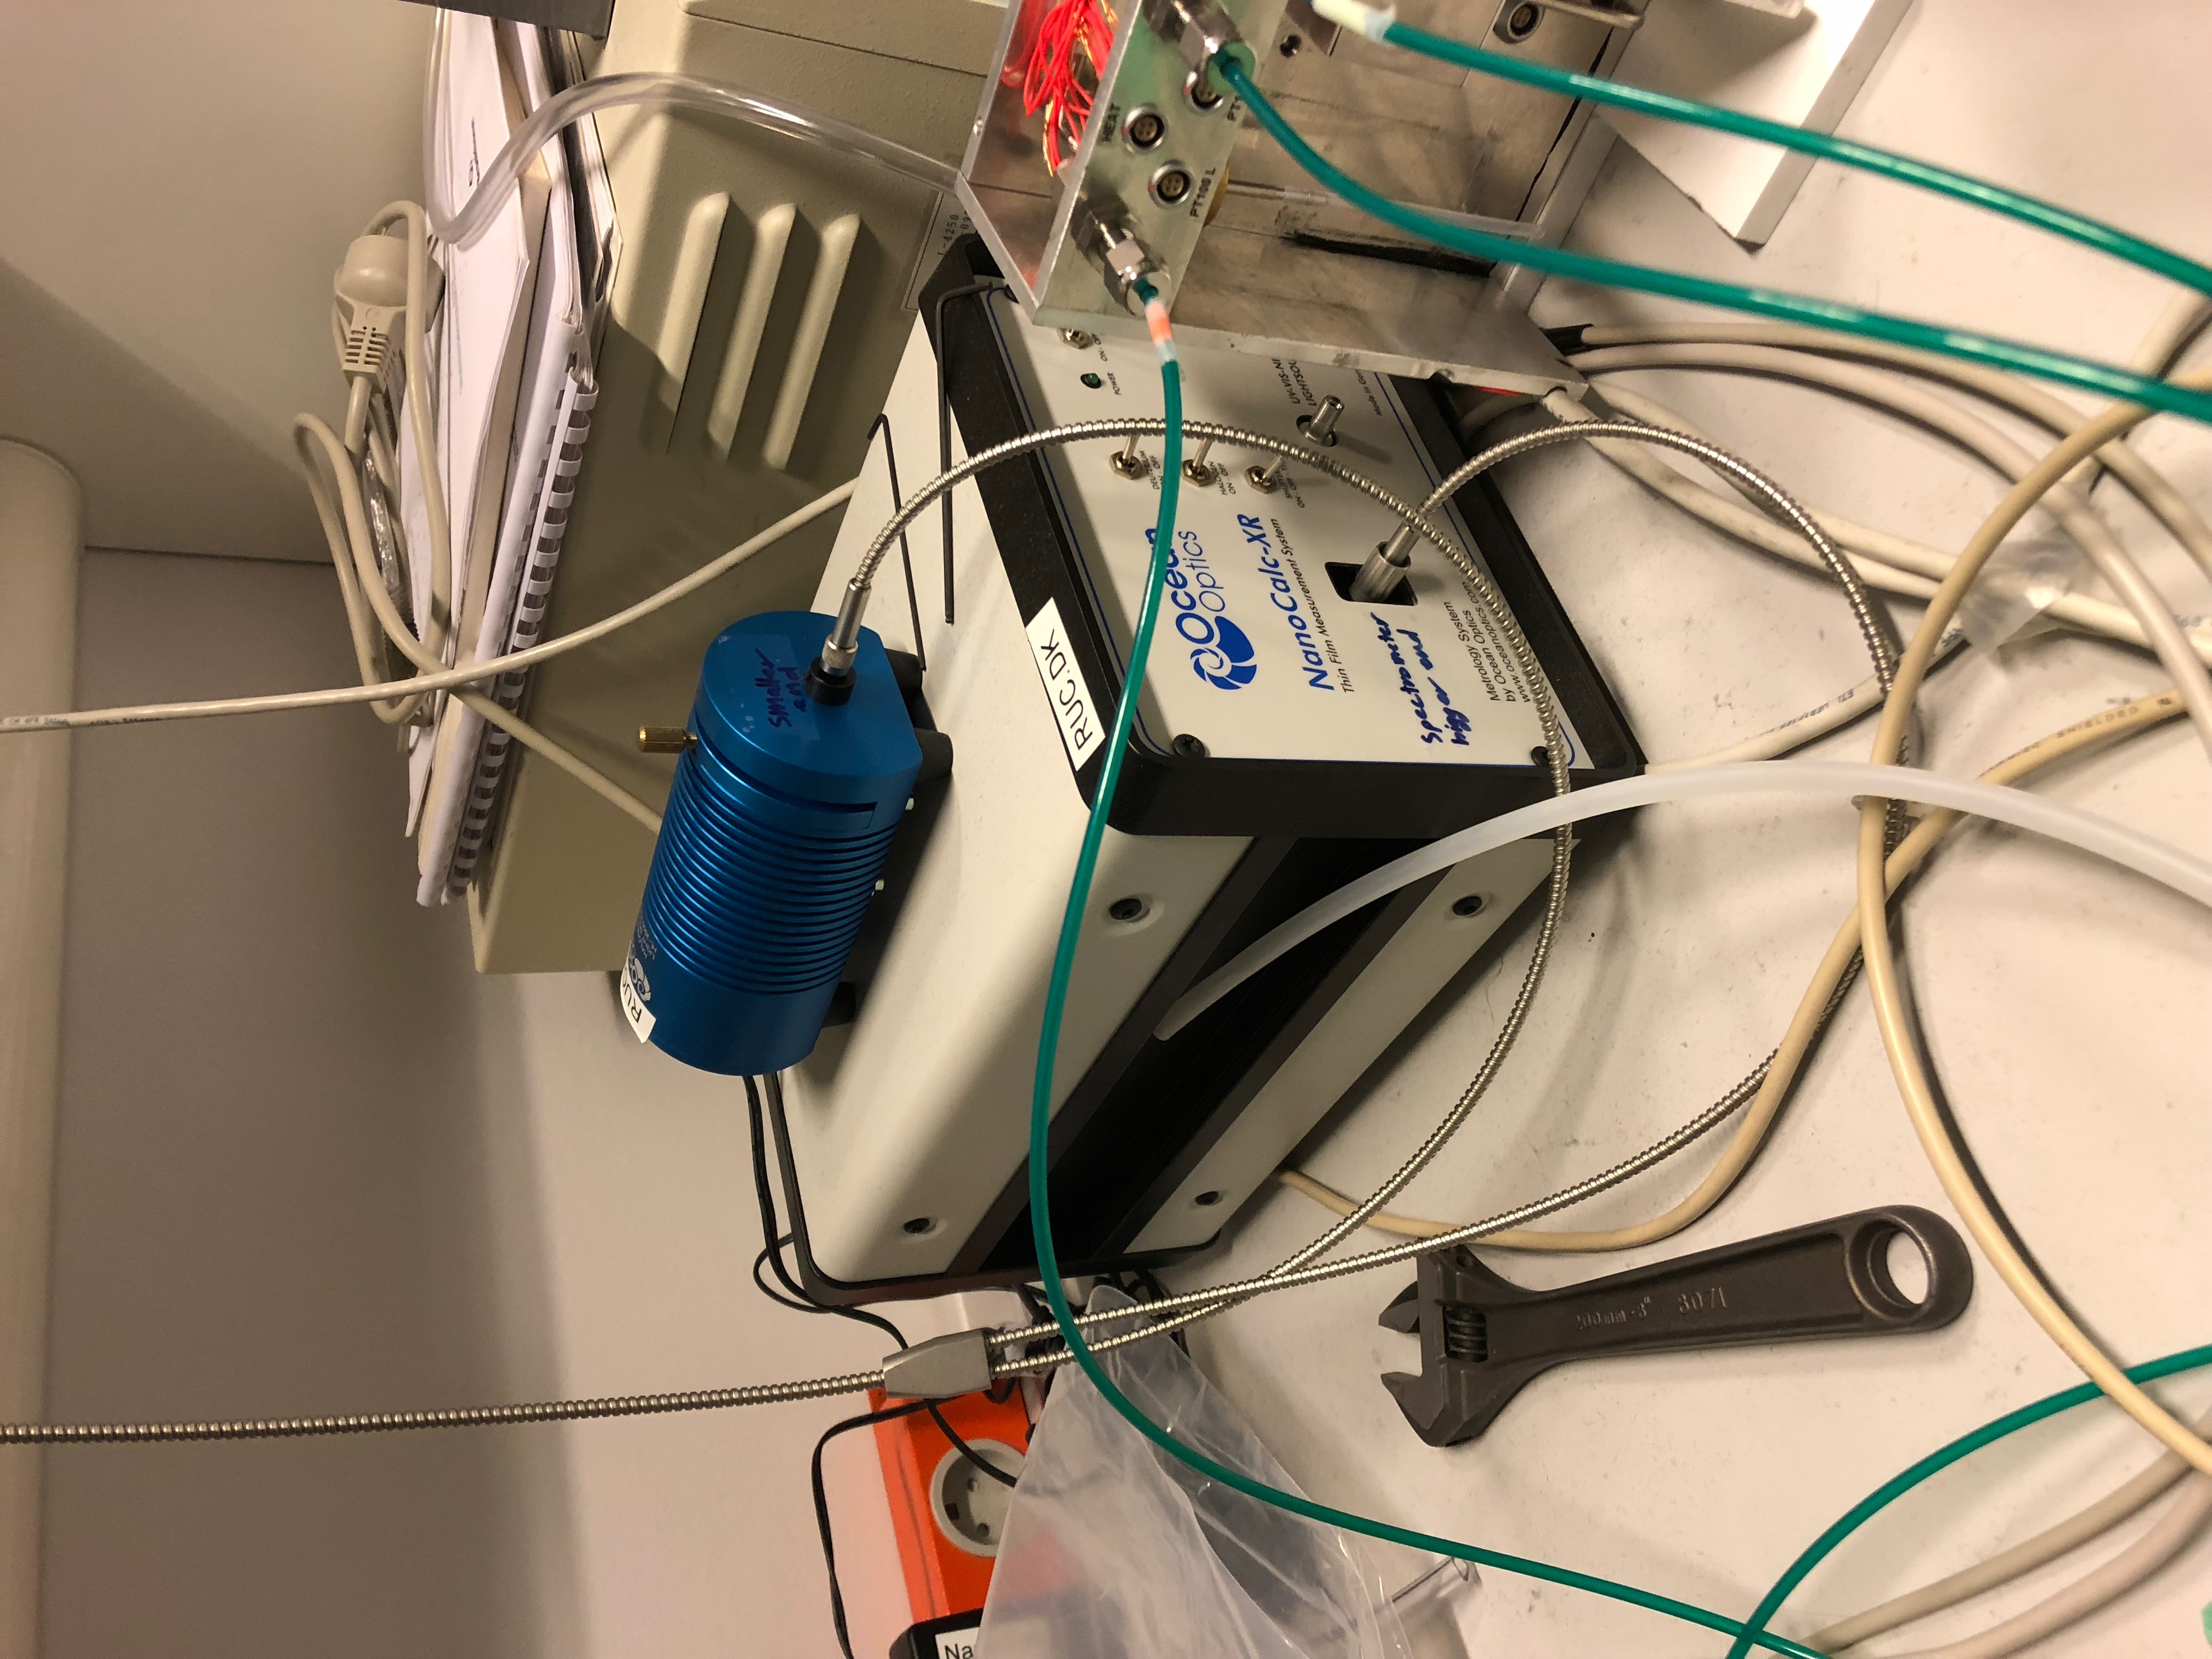
\includegraphics[scale=0.04,angle=-90]{setup2.JPG}
	\end{figure}
	\end{minipage}

	\end{frame}
	
	\begin{frame}{Components Cont.}
	\begin{minipage}{0.47\textwidth}
	\begin{figure}
	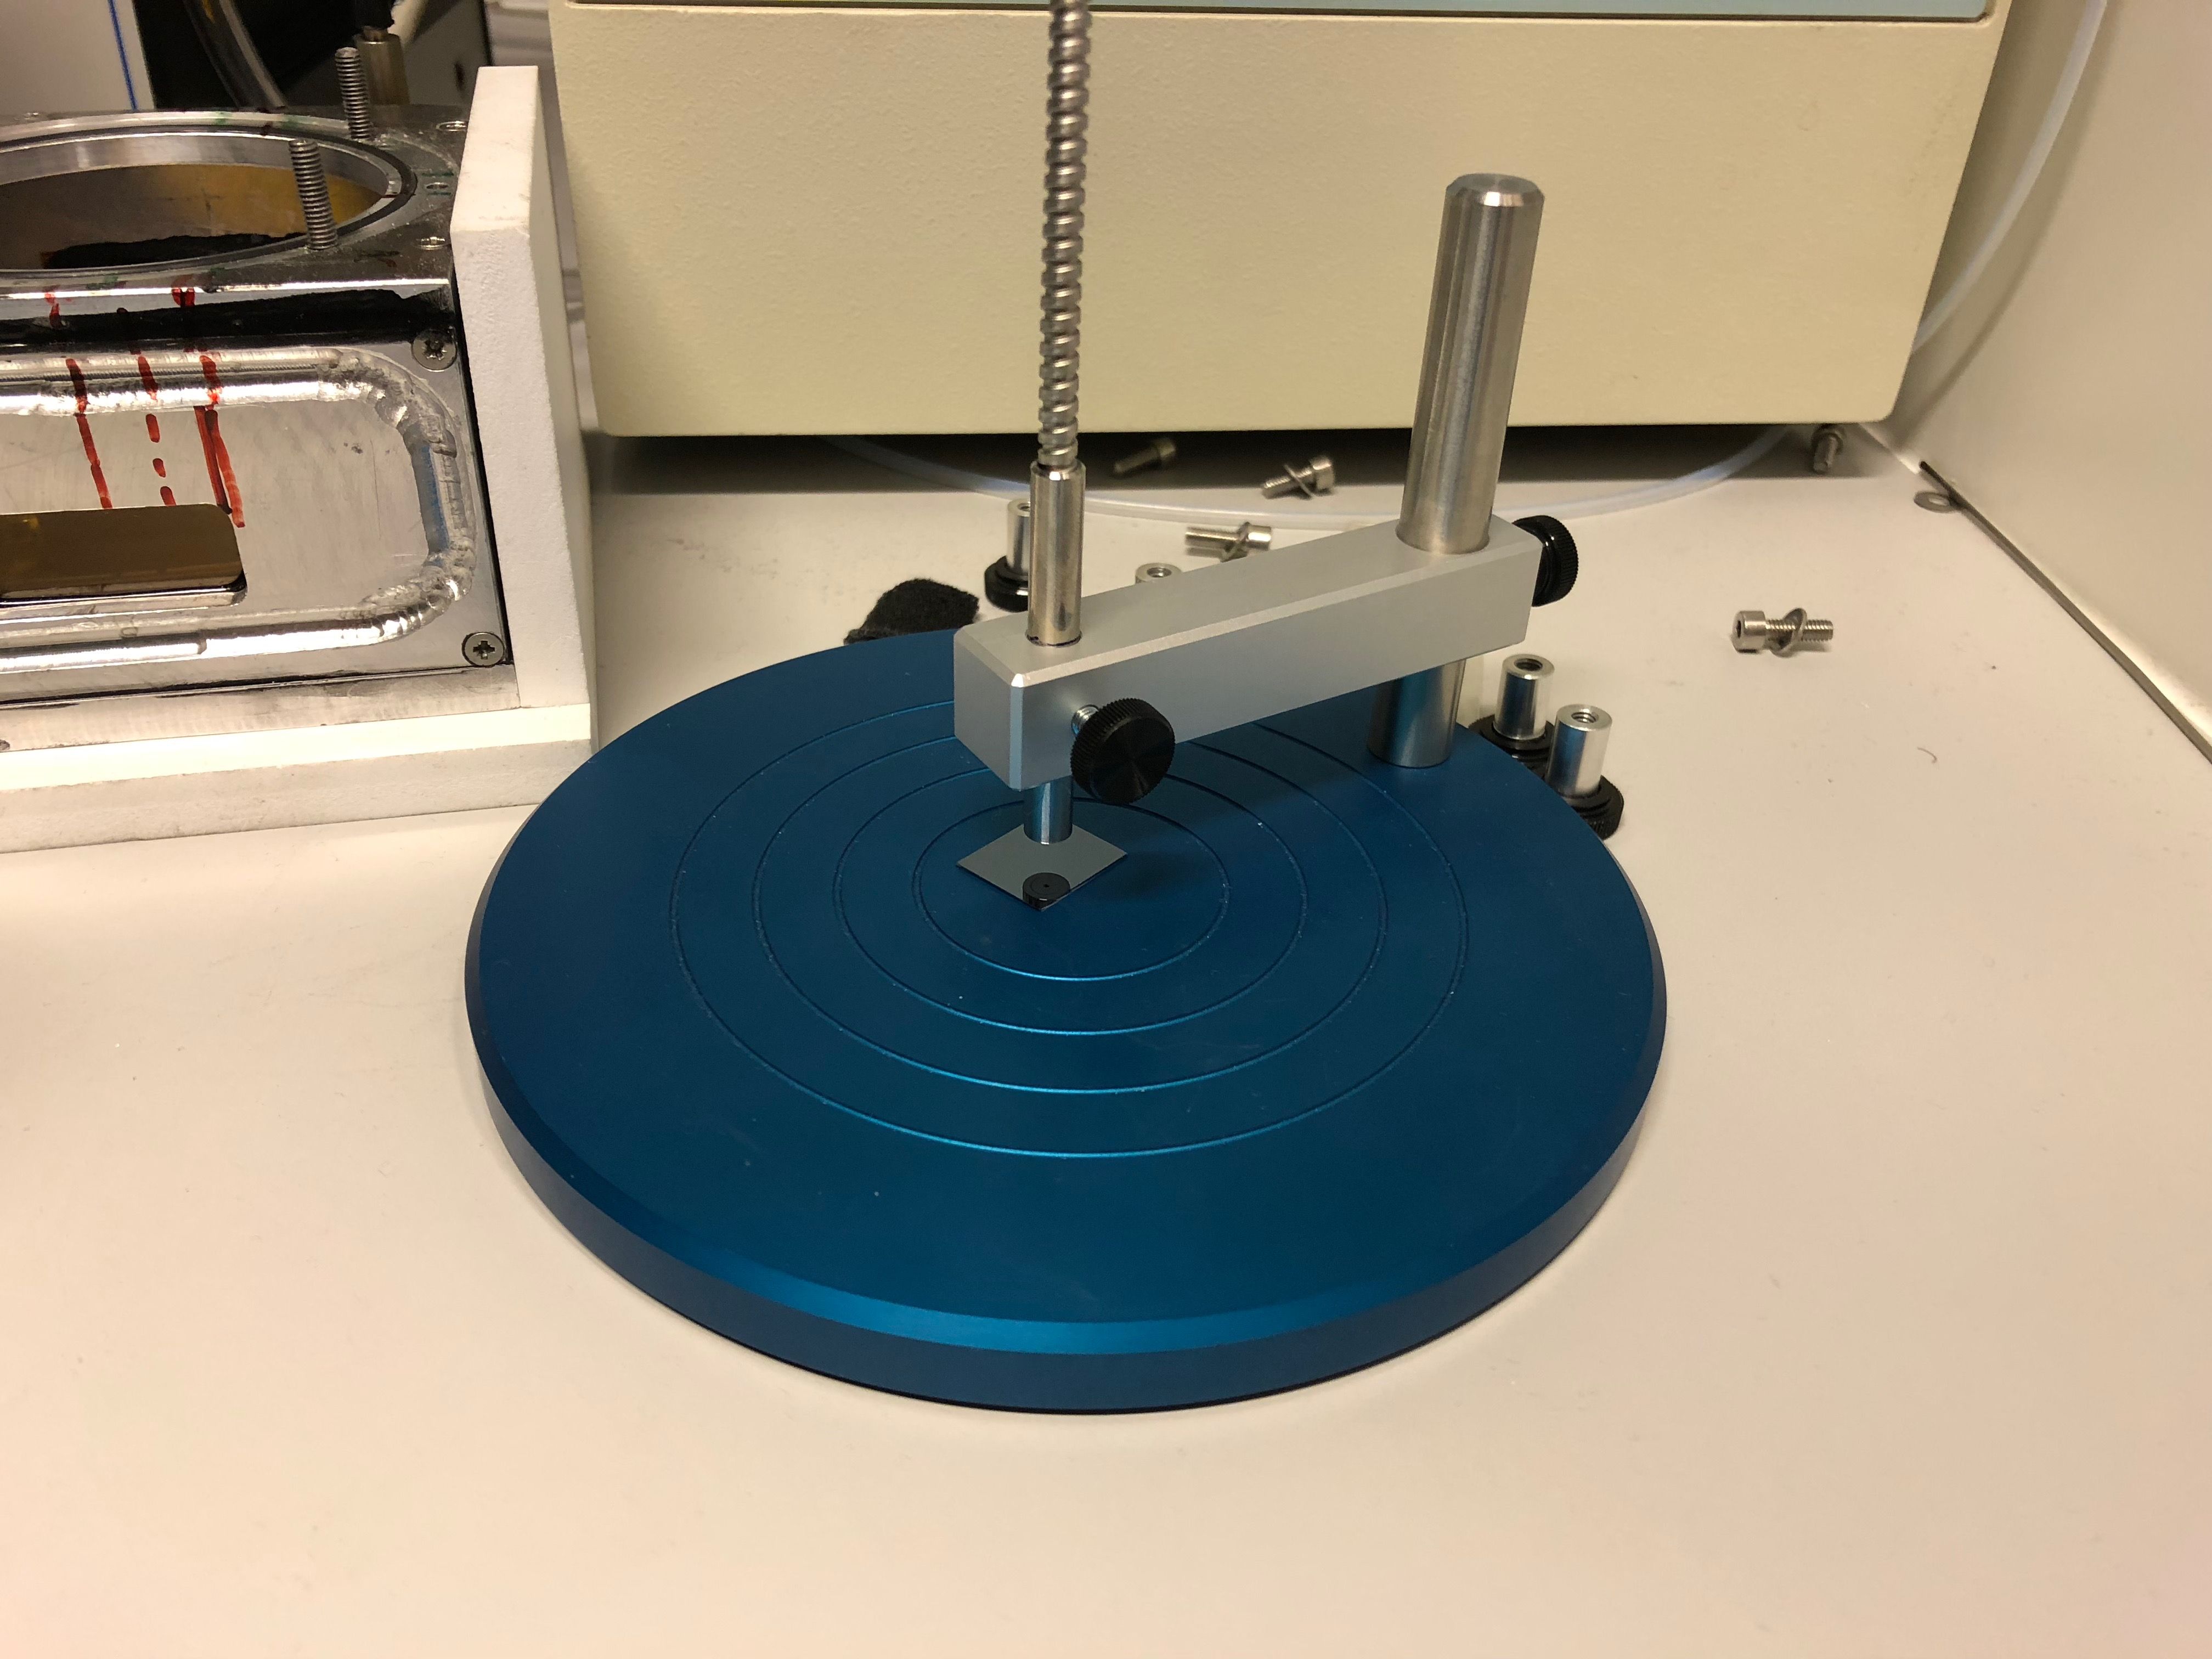
\includegraphics[scale=0.04]{setup3.JPG}
	\end{figure}
	\end{minipage}
	\begin{minipage}{0.5\textwidth}
	\begin{figure}
	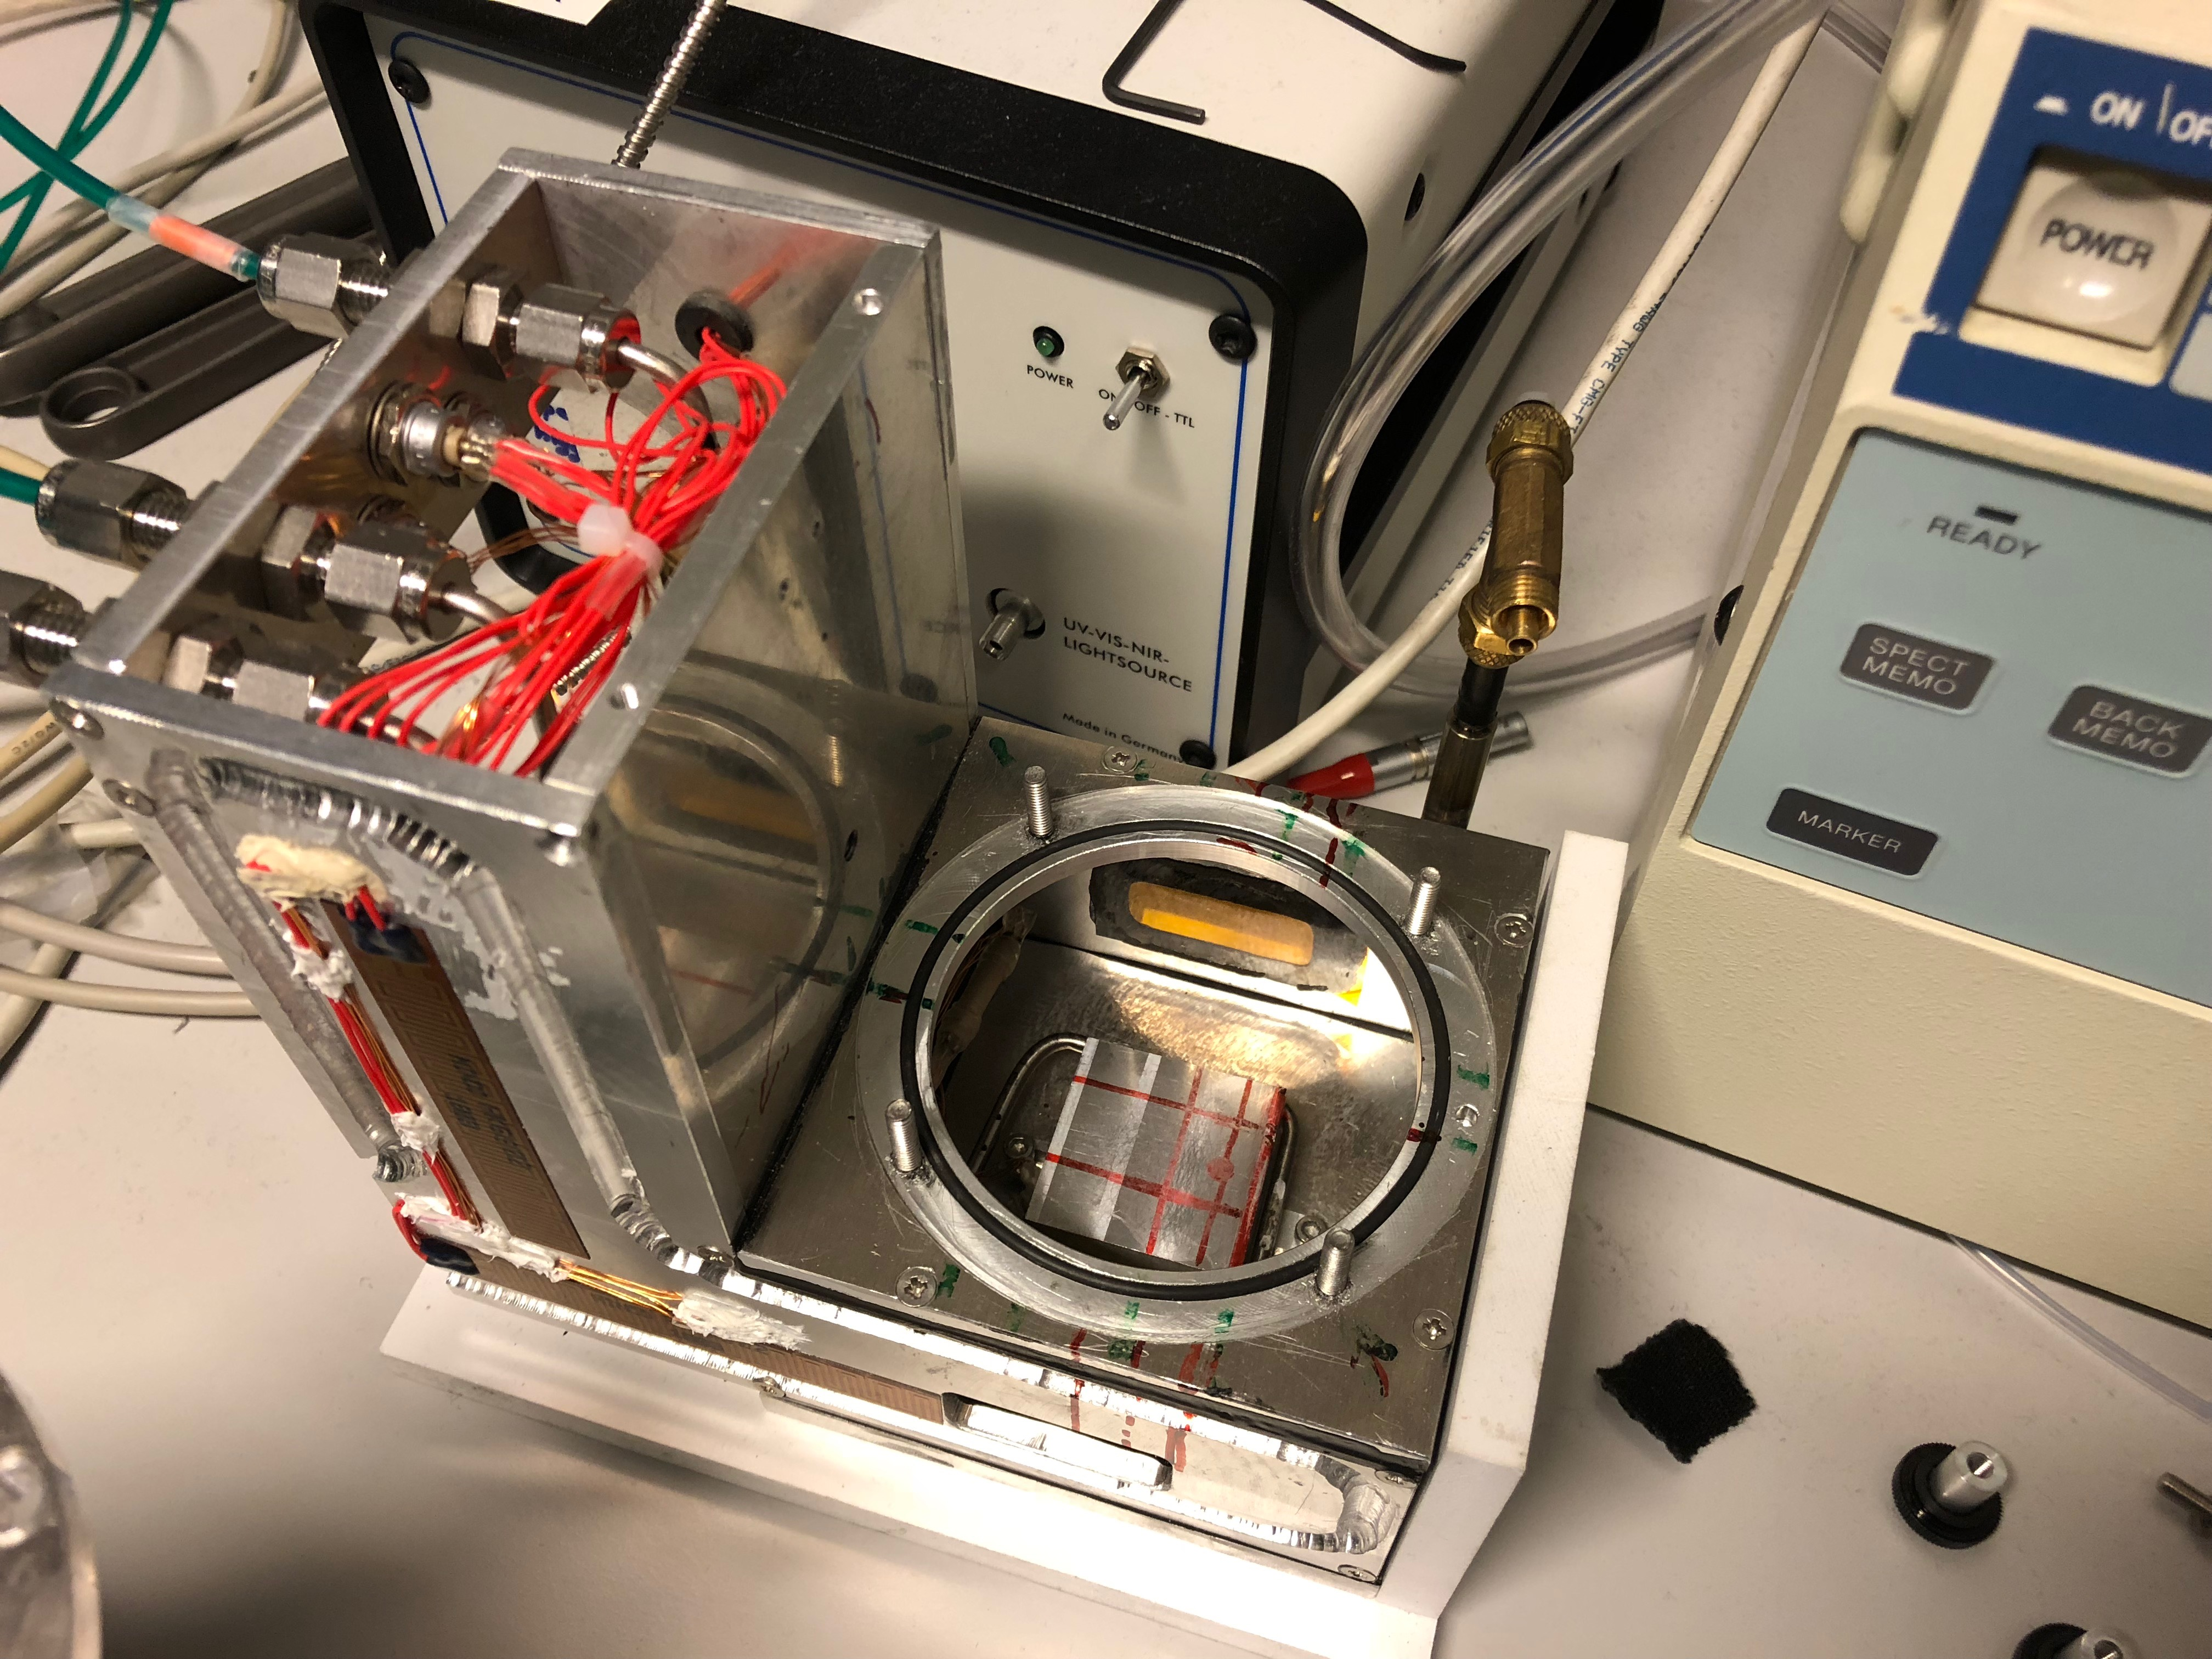
\includegraphics[scale=0.04]{setup4.JPG}
	\end{figure}
	\end{minipage}
	\end{frame}
	
	\begin{frame}{NanoCalc Software}
	
	\begin{figure}
	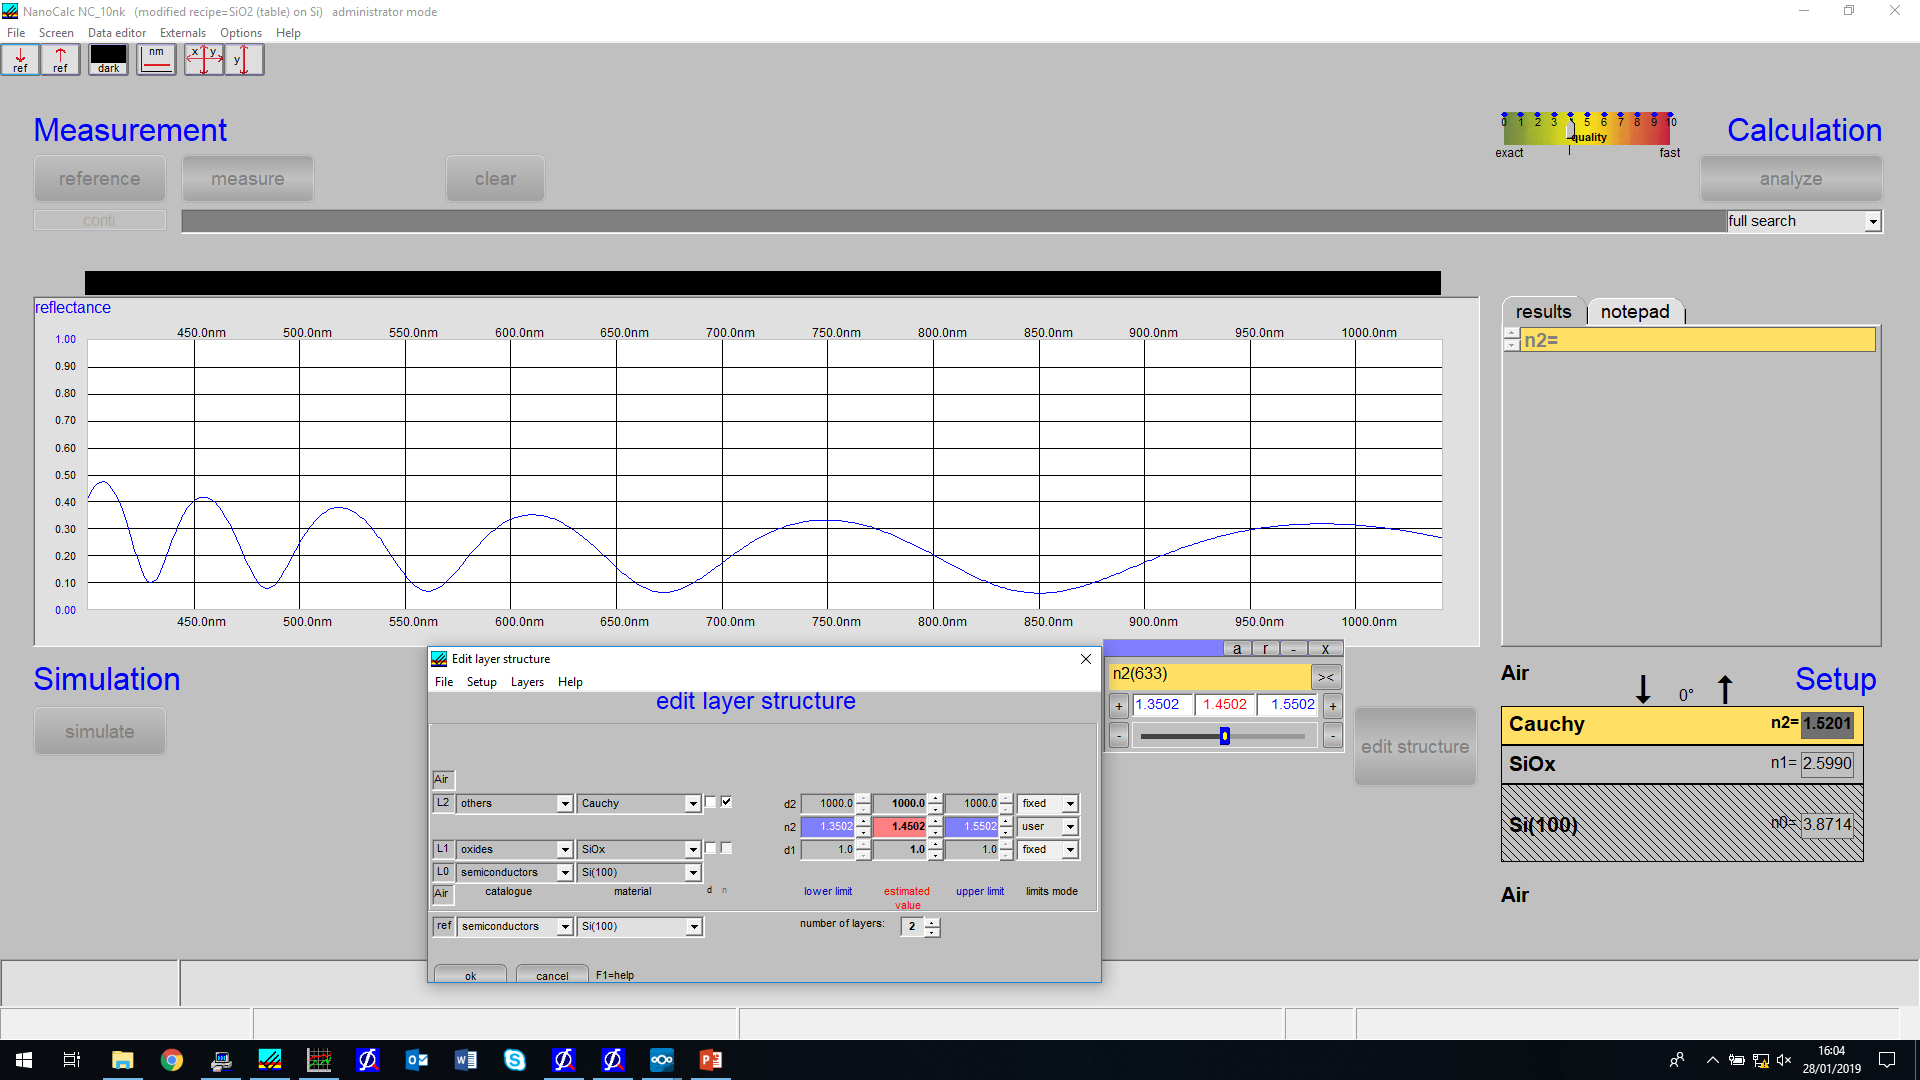
\includegraphics[width=\textwidth]{nanocalc.png}
	\end{figure}
	
	\end{frame}
	
	\section{Preliminary Models}
	
	\begin{frame}{Fresnel Equations - Substrate}
	
	\end{frame}
	
	\begin{frame}{Fresnel Equations - One layer}
	
	\begin{figure} 
		 \begin{center}
		   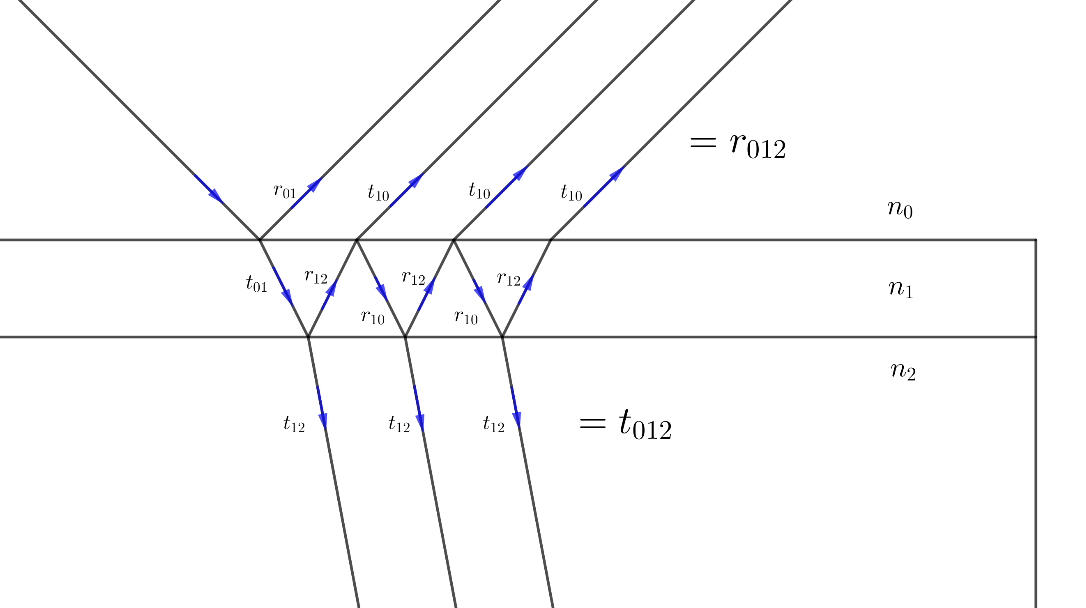
\includegraphics[width=\textwidth]{figreflre.png}
		 \end{center}
	\end{figure}
	\begin{align*}
	r_{012} = &r_{01} + t_{01}t_{10}r_{12}\exp(-i2\beta) + t_{01}t_{10}r_{10}r_{12}^2\exp(-i4\beta)+ \\ &t_{01}t_{10}r_{10}^2r_{12}^3\exp(-i6\beta)+ \cdots
	\end{align*} 
	
	\end{frame}
	
	\begin{frame}{Fresnel Equations - One layer}
	
	\begin{minipage}{0.47\textwidth}
	
	\begin{equation*} \label{eq:r012big}
	r_{012}=r_{01}+\frac{t_{01}t_{10}r_{12}\exp(-i2\beta)}{1-r_{10}r_{12}\exp(-i2\beta)}
	\end{equation*}
		
	\begin{equation*}\label{eq:2layerreflect}
	r_{012}= \frac{r_{01}+r_{12}\exp(-i2\beta)}{1+r_{01}r_{12}\exp(-i2\beta)}
	\end{equation*} 
	\end{minipage}
	\begin{minipage}{0.5\textwidth}
	\begin{equation*}
	\beta=\frac{2\pi d_1}{\lambda} n_1\cos(\theta_1)
	\end{equation*}
	\end{minipage}	
	\end{frame}
	
	\begin{frame}{Fresnel equations - multilayers}
	
	\begin{figure}
	\centering
	\begin{minipage}{0.5\textwidth}
	\centering
	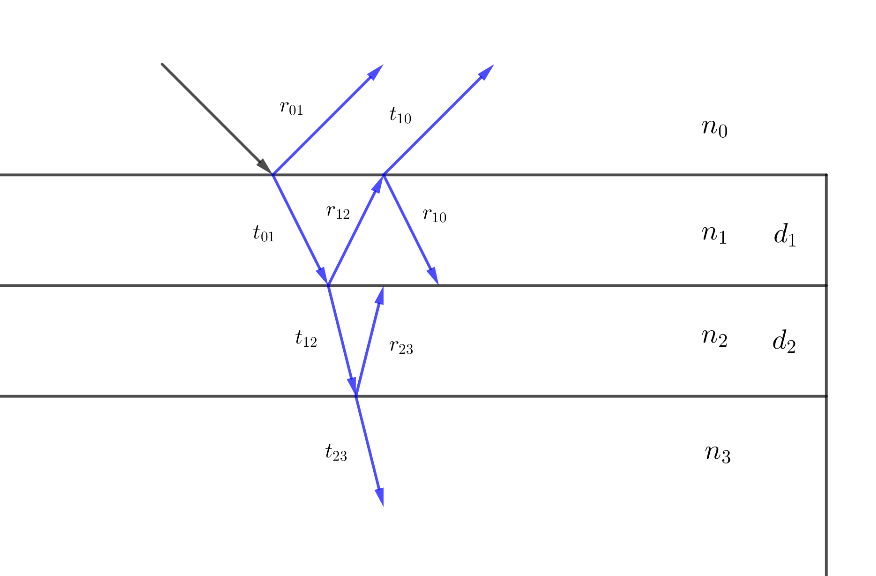
\includegraphics[scale=0.2]{figmulti1re.png}
	\end{minipage}\quad
	\begin{minipage}{0.5\textwidth}
	\begin{figure}
	\centering
	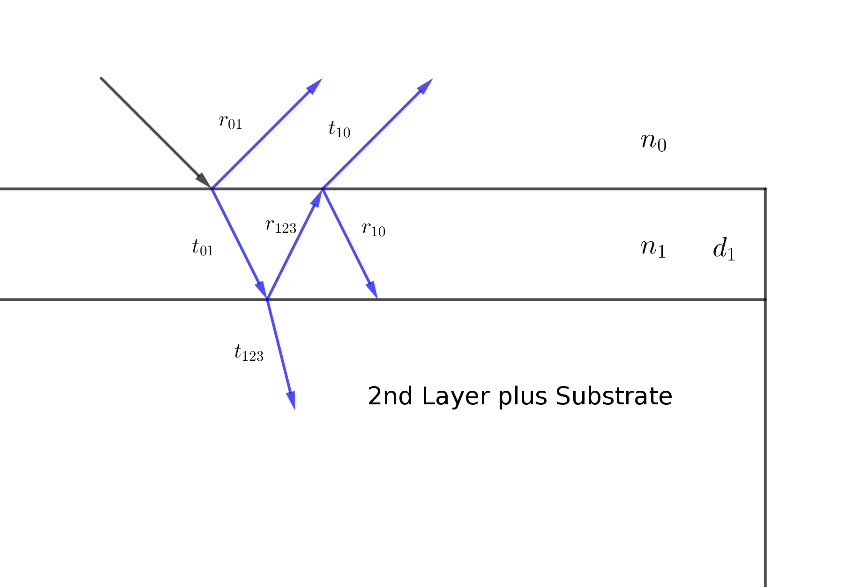
\includegraphics[scale=0.2]{figmulti2re.png}
	\end{figure}
	\end{minipage}
	\end{figure}
	
	\end{frame}
	
	\begin{frame}{Fresnel equations - multilayers Cont.}
	
	\begin{minipage}{0.47\textwidth}
	\begin{equation*}
	r_{123}= \frac{r_{12}+r_{23}\exp(-i2\beta_2)}{1+r_{12}r_{23}\exp(-i2\beta_2)}
	\end{equation*}
	
	\begin{equation*}
	r_{0123}= \frac{r_{01}+r_{123}\exp(-i2\beta_1)}{1+r_{01}r_{123}\exp(-i2\beta_1)}
	\end{equation*}
	\end{minipage}
	\begin{minipage}{0.5\textwidth}
		\begin{equation*}
		\beta=\frac{2\pi d}{\lambda} n\cos(\theta)
		\end{equation*}
	\end{minipage}
	\end{frame}
	
	\begin{frame}{Homopolymer Results}
	
	\end{frame}
\end{document}